\documentclass[border=10pt]{standalone}

\usepackage{tikz}
\usepackage{tikzsymbols}
\usetikzlibrary{calc,patterns,shapes.geometric}

\def\centerarc[#1](#2)(#3:#4:#5){\draw[#1] ($(#2)+({#5*cos(#3)},{#5*sin(#3)})$) arc (#3:#4:#5);}

\begin{document}
	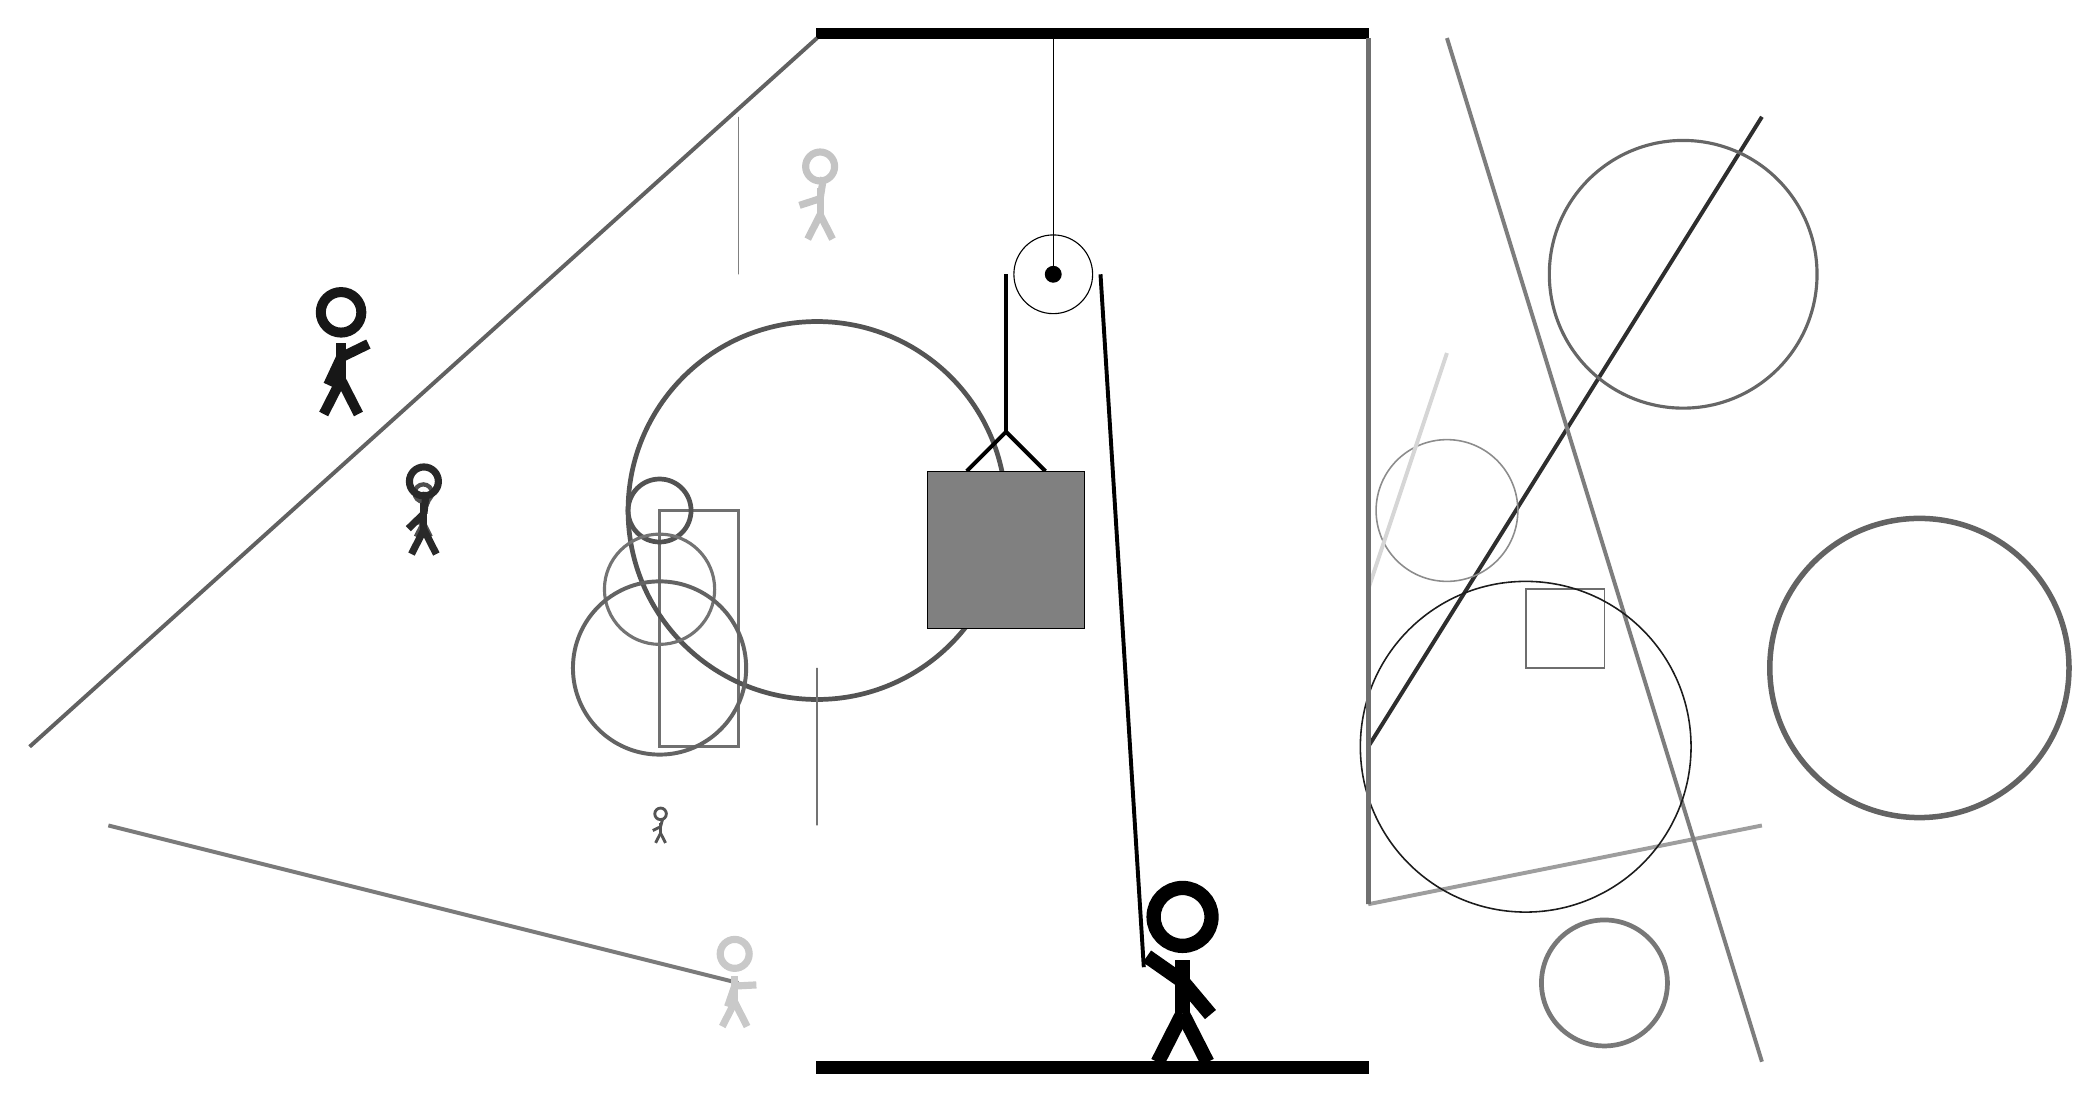
\begin{tikzpicture}
		%%%%% START %%%%%
		
		\draw[fill=black] (-2, 10) rectangle (5, 10.125);
		
		\draw (1, 7) circle (0.5);
		\draw[fill=black] (1, 7) circle (0.1);
		\draw (1, 10) -- (1, 7);
		
		\draw[line width=0.4mm, color=black!56] (-4, 4) rectangle (-3, 1);
		
		\draw [line width=0.6mm, color=black!68](-4, 4) circle (0.4);
		\node[line width=0.2mm, color=black!67] at (-4, 0) {\Strichmaxerl[2][26][75]};
		\draw [line width=0.6mm, color=black!67](-2, 4) circle (2.4);
		\draw[line width=0.5mm, color=black!82](10, 9) -- (5, 1);
		
		\draw [line width=0.4mm, color=black!55](-4, 3) circle (0.7);
		\draw[line width=0.5mm, color=black!52](-3, -2) -- (-11, 0);
		\draw[line width=0.2mm, color=black!57] (7, 3) rectangle (8, 2);
		\draw [line width=0.2mm, color=black!45](6, 4) circle (0.9);
		
		\draw [line width=0.6mm, color=black!53](8, -2) circle (0.8);
		\draw[line width=0.5mm, color=black!38](10, 0) -- (5, -1);
		
		\node[line width=0.5mm, color=black!69] at (-7, 4) {\Strichmaxerl[3][73][66]};
		\draw[line width=0.2mm, color=black!55] (-2, 0) rectangle (-2, 2);
		
		\node[line width=0.6mm, color=black!23] at (-2, 8) {\Strichmaxerl[5][18][81]};
		\draw [line width=0.7mm, color=black!61](12, 2) circle (1.9);
		\node[line width=0.6mm, color=black!84] at (-7, 4) {\Strichmaxerl[5][44][84]};
		
		\draw [line width=0.5mm, color=black!61](-4, 2) circle (1.1);
		\draw[line width=0.5mm, color=black!51](6, 10) -- (10, -3);
		\draw[line width=0.5mm, color=black!16](6, 6) -- (5, 3);
		\draw[line width=0.2mm, color=black!50] (-3, 7) rectangle (-3, 9);
		\draw [line width=0.4mm, color=black!60](9, 7) circle (1.7);
		\node[line width=0.7mm, color=black!91] at (-8, 6) {\Strichmaxerl[7][65][26]};
		\node[line width=0.3mm, color=black!21] at (-3, -2) {\Strichmaxerl[5][71][3]};
		\draw [line width=0.2mm, color=black!89](7, 1) circle (2.1);
		\draw[line width=0.5mm, color=black!62](-2, 10) -- (-12, 1);
		
		\draw[line width=0.6mm, color=black!56] (5, 10) rectangle (5, -1);
		
		\draw[line width=0.5mm] (-0.1, 4.5) -- (0.4, 5.0) -- (0.9, 4.5);
		\draw[fill=black!50] (-0.6, 4.5) rectangle (1.4, 2.5);
		
		\draw[line width=0.5mm] (0.4, 7) -- (0.4, 5.0);
		\centerarc[line width=0.5mm](1, 7)(0:180:0.6);
		\draw[line width=0.5mm](1.6, 7) -- (2.15, -1.8);
		
		\node at (2.6, -1.9) {\Strichmaxerl[10][-35][-50]};
		
		\draw[fill=black] (-2, -3) rectangle (5, -3.15);
		
		%%%%% END %%%%%
	\end{tikzpicture}
\end{document}